\chapter{API desenvolvida} \label{cap:proposta}

  A criação de uma API RESTFul para o contexto deste trabalho é adequada, pois promove baixo acoplamento
  entre os componentes da aplicação, não sobrecarregando o ``Empurrando Juntos'' com funcionalidades genéricas
  para as conversas e de agrupamento dos usuários,
  permitindo a reutilização dos serviços de clusterização por qualquer
  outra aplicação que já existe ou que venha a ser criada, tanto \textit{web} como \textit{mobile}.
  
  A seção \ref{requirements} apresenta os requisitos identificados para a solução.
  A seção \ref{architecture} apresenta a descrição da arquitetura definida para a solução.

\section{Requisitos da solução} \label{requirements}

    Considerando as necessidades do ``Empurrando Juntos'',
    foram identificados requisitos funcionais e não funcionais da aplicação,
    que são apresentados a seguir.

    \subsection*{Requisitos Funcionais} \label{functional_requirements}

    Uma avaliação do escopo da plataforma ``Empurrando Juntos'' permitiu o levantamento de características desejadas do sistema e,
    consequentemente, alguns requisitos associados, que foram sumarizados na Tabela \ref{tab:requisitos}.

    \begin{table}[h!]
    \centering
    \caption{Requisitos funcionais de alto nível da aplicação.}
    \label{tab:requisitos}
    \begin{tabular}{@{}cl@{}}
    \toprule
    \textbf{Característica}                      & \multicolumn{1}{c}{\textbf{Requisito}}                                                                                                \\ \midrule
    \multirow{5}{*}{Gerenciamento de Usuário}    & O sistema deve permitir o cadastro de usuários                                                                                        \\
						& O sistema deve permitir a alteração de usuários                                                                                       \\
						& \begin{tabular}[c]{@{}l@{}}O sistema deve permitir a autenticação de usuários \\ cadastrados na plataforma\end{tabular}			\\
						&  \begin{tabular}[c]{@{}l@{}}O sistema deve permitir a autenticação de usuários \\ cadastrados no Facebook\end{tabular}                     \\ \midrule
    \multirow{3}{*}{Gerenciamento de Conversa}   & O sistema deve permitir o cadastro de conversas                                                                                       \\
						& O sistema deve permitir a alteração de conversas                                                                                      \\
						& O sistema deve permitir a exclusão de conversas                                                                                       \\ \midrule
    \multirow{4}{*}{Gerenciamento de Comentário} & O sistema deve permitir o cadastro de comentários em conversas                                                                        \\
						& O sistema deve permitir a alteração de comentários                                                                                    \\
						& O sistema deve permitir a exclusão de comentários                                                                                     \\ 
						& O sistema deve permitir que o usuário vote em comentários                                                                             \\ \midrule
    Agrupamento de usuários                      & \begin{tabular}[c]{@{}l@{}}O sistema deve permitir a 
						  visualização dos usuários agrupados \\ de acordo com os votos dados\end{tabular} \\ \bottomrule
      \end{tabular}
	\end{table}
	  
      
    \subsection*{Requisitos não funcionais}	\label{non_functional_requirements}	
	
    Todos os serviços da API serão providos para a plataforma por meio de uma interface HTTP/HTTPS utilizando o estilo arquitetural REST.
%     A API deve possibilitar a escolha do módulo matemático a ser utilizado, considerando as opções previamente implementadas.

    A autenticação e autorização das aplicações, e seus respectivos usuários devem ser realizadas por meio de JWT \textit{tokens}.

    A tecnologia definida para implementação da solução proposta foi a linguagem Python juntamente com os \textit{frameworks}
    Django e Django Rest Framework, utilizando o banco de dados PostgreSQL.

    Outro aspecto importante para esta aplicação é a questão da manutenibilidade, pois como será um software livre, a solução
    deve ser desenvolvida de uma maneira que seja possível evoluir facilmente pela da comunidade.
    Com isto em mente, foram definidos os seguintes padrões para o desenvolvimento da aplicação, considerando as tecnologias definidas:
    utilização do PEP8 \footnotemark como folha de estilos e a utilização da especificação JSON API \footnotemark para formatação das respostas da API.
    \footnotetext{Folha de estilos PEP8. Disponível em \href{https://www.python.org/dev/peps/pep-0008/}{https://www.python.org/dev/peps/pep-0008}.}
    \footnotetext{Especificação JSON API. Disponível em \href{http://jsonapi.org/}{http://jsonapi.org}.}

\section{Arquitetura da solução} \label{architecture}
    
    Considerando o objetivo do trabalho de implementar uma API capaz de trabalhar com 
    módulos matemáticos plugáveis, a solução proposta está representada na Figura \ref{fig:pentano}, 
    na qual são indicados os dois módulos tratados na solução: os módulos API e Matemático. Estes
    dois módulos em conjunto com a aplicação cliente formam o sistema por completo que será denominado neste trabalho
    de \textit{Pentano}.
    
    \begin{figure}[h!]
    \centering
    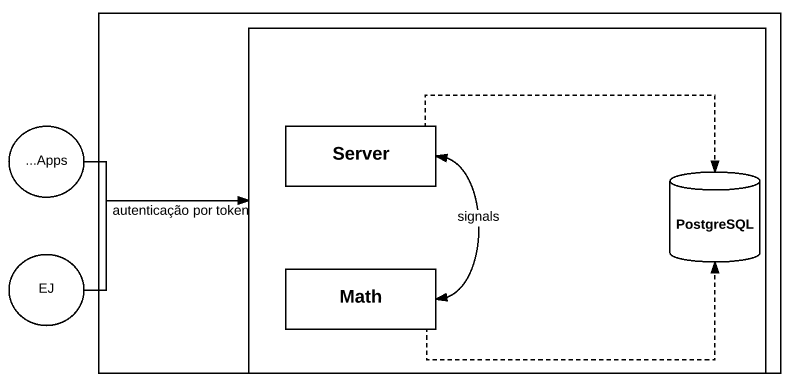
\includegraphics[scale=0.7]{figuras/esquema_pentano.png}
    \caption{Estrutura do Pentano}
    \label{fig:pentano}
    \end{figure}
    
    A arquitetura proposta é definida pelo módulo de API, o módulo Matemático
    e o protocolo de comunicação entre esses dois módulos, como ilustra a Figura \ref{fig:pentano}.
    
    O módulo de API é uma aplicação independente que contém a lógica para o gerenciamento das conversas e usuários e
    serve como ponto de entrada para o sistema.
    
    Os módulos matemáticos também são aplicações independentes que implementam a interface definida no protocolo
    para se comunicarem com a API, de modo que seja possível criar vários módulos matemáticos utilizando algoritmos diferentes.
    Os módulos matemáticos encapsulam a lógica de agrupar os usuários com base nos votos obtidos.
    
    Para a comunicação entre a API e os módulos matemáticos escolhidos, foi utilizada
    uma plataforma de execução de tarefas assíncronas, o Celery \footnotemark, que é uma aplicação
    madura, estável, bem acolhida pela comunidade e que é de fácil integração com projetos em Python.
    O Celery funciona a partir da definição de tarefas que podem ser executadas de forma assíncrona
    e utiliza um \textit{message broker}, que é uma plataforma intermediária
    entre duas aplicações para troca de mensagens, para enfileirar e delegar as tarefas para execução.
    
    Essa ferramenta em conjunto com uma interface de tarefas definidas formam
    a comunicação entre a API e o módulo responsável pela clusterização. 
    Uma visão geral do protocolo pode ser vista na Figura \ref{fig:protocolo}.
    \footnotetext{http://www.celeryproject.org/}

    \begin{figure}[bt!]
    \centering
    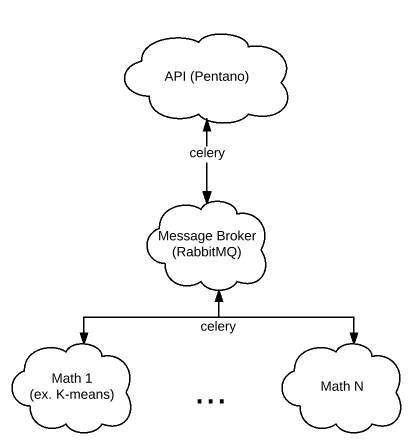
\includegraphics[scale=0.6]{figuras/protocolo.png}
    \caption{Esquema de comunicação entre os módulos de API e Matemático}
    \label{fig:protocolo}
    \end{figure}
    
%     Fica a cargo da implantação do sistema de associar a API desenvolvida neste trabalho com algum módulo matemático 
%     existente ou novo.
    
    \subsection{Módulo de API}

	O módulo de API é responsável por gerenciar as conversas, comentários, votos
	e cuidar de todos os aspectos da autenticação das aplicações. 

	Para o módulo de API, foram mapeadas as entidades principais e os relacionamentos entre elas. 
	As principais entidades que foram identificadas são Usuário, Conversa e Comentário. Um usuário pode criar
	conversas e comentários para cada conversa e participar de outras conversas, criadas por outros usuários.
	A participação de um usuário em uma conversa é dada pelo ato de criação de comentários naquela conversa ou
	no ato de votar em um comentário de uma conversa. Esse mapeamento é ilustrado na Figura \ref{fig:entidades}.

	\begin{figure}[h!]
	\centering
	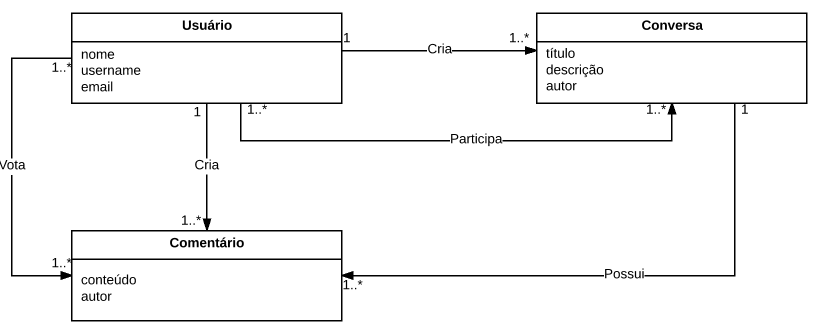
\includegraphics[scale=0.5]{figuras/entidades.png}
	\caption{Relacionamento das principais entidades da API}
	\label{fig:entidades}
	\end{figure}

	Como o \textit{framework} Django foi escolhido como tecnologia de implementação da API,
	a arquitetura proposta foi pensada valendo-se de 
	recursos providos pela própria arquitetura do \textit{framework}.
	No Django, uma aplicação web é abstraída como um projeto, e um projeto é composto por uma coleção de aplicações
	(ou, de forma abreviada, \textit{apps}) independentes, que
	são pacotes Python que proveem um conjunto de funcionalidades relacionadas e podem ser reutilizados \cite{django_apps}.

	Portanto, toda a solução foi componentizada utilizando \textit{apps} do 
	Django. Considerando os requisitos funcionais e não funcionais da solução, especificados anteriormente, a arquitetura da solução foi definida 
	conforme a Figura \ref{fig:arquitetura_api}, onde no módulo \textit{API} temos dois \textit{apps} independentes, um responsável
	por cuidar de toda parte de autenticação da aplicação (\textit{app} de contas) e o outro para gerenciar as entidades apresentadas na
	Figura \ref{fig:entidades} (\textit{app} de conversas). 

	\begin{figure}[h!]
	\centering
	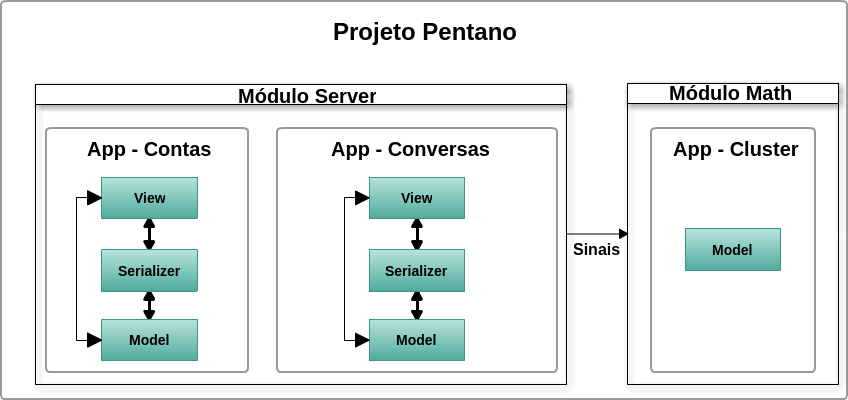
\includegraphics[scale=0.8]{figuras/arquitetura_api.png}
	\caption{Arquitetura de \textit{apps} da API}
	\label{fig:arquitetura_api}
	\end{figure}

	Para cada \textit{app} foi definida uma arquitetura
	em 3 camadas: \textit{models}, \textit{views} e \textit{serializers}.
	A camada \textit{view} recebe e responde as requisições provenientes do cliente.
	A camada \textit{serializer} é responsável pelo tratamento e formatação dos dados das \textit{models}
	para renderização em JSON, seguindo a especificação JSON API.
	Por fim, a camada \textit{model} contém aspectos negociais relacionados a cada uma das entidades definidas na 
	Figura \ref{fig:entidades}.
	
	Para não acoplar as \textit{models} comunicando diretamente com o módulo matemático,
	a comunicação é feita a partir de uma camada de sinais, que são acionados quando alguma ação ocorre nas \textit{models}.
	Esta camada de sinais é implementada utilizando a arquitetura de sinais do Django.
	As seguintes ações possuem sinais registrados:
	
	\begin{itemize}
	 \item Criação de uma nova conversa;
	 \item Criação de um novo comentário;
	 \item Novos votos em um comentário de uma conversa.
	\end{itemize}

    
%     \vfill
%     \pagebreak
    
    \subsection{Módulo matemático}
	
	O módulo matemático é responsável por receber os votos de uma conversa
	e gerar os grupos de usuários (\textit{clusters}) de acordo com o algoritmo implementado no respectivo módulo.

	Para estabelecer comunicação com a API, o módulo matemático deve seguir as seguintes diretrizes:
	\begin{itemize}
	  \item Deve ser uma aplicação que possua o Celery configurado;
	  \item Deve implementar as 4 tarefas especificadas na Tabela \ref{tab:tasks};
	  \item Deve garantir que as tarefas estão registradas no Celery com os nomes apresentados na Tabela \ref{tab:tasks}.
	  \item Deve garantir que o Celery esteja configurado para escutar no mesmo \textit{message broker} que a API.
	\end{itemize}
	
	
	Considerando que o módulo matemático implemente todas as diretrizes definidas acima, a comunicação é realizada com 
	os seguintes passos:
	  
	\begin{enumerate}
	\item O cliente realiza uma das requisições relacionada a uma das 4 tarefas da Tabela \ref{tab:tasks};
	\item A API processa a requisição e enfileira a tarefa no \textit{message broker};
	\item O Celery executando no projeto onde encontra-se o módulo matemático captura a chamada da tarefa através do mesmo \textit{message broker} e 
	executa a tarefa especificada;
	\item O módulo matemático retorna o resultado de execução da tarefa;
	\item A API recebe o resultado retornado do módulo matemático, identificando o sucesso ou a falha da tarefa executada.
	\end{enumerate}

	\begin{table}[h!]
	\centering
	\caption{Interface de comunicação entre a API e os módulos matemáticos}
	\label{tab:tasks}
	  \begin{tabular}{@{}lll@{}}
	  \multicolumn{1}{c}{\textbf{Tarefa}}                                                & \multicolumn{1}{c}{\textbf{Parâmetros}}                                                                               & \multicolumn{1}{c}{\textbf{Retorno}} \\ \midrule
	  \begin{tabular}[c]{@{}l@{}}Adicionar nova conversa \\ (pentano.new\_conversation)\end{tabular} & Identificador da conversa                                                                                             & Confirmação de Sucesso               \\ \midrule
	  \begin{tabular}[c]{@{}l@{}}Adicionar novo comentário \\ (pentano.add\_comment)\end{tabular}    & \begin{tabular}[c]{@{}l@{}}Identificador da conversa\\ Identificador do comentário\\ Texto do comentário\end{tabular} & Confirmação de Sucesso               \\ \midrule
	  \begin{tabular}[c]{@{}l@{}}Adicionar novo voto\\ (pentano.add\_votes)\end{tabular}             & \begin{tabular}[c]{@{}l@{}}Identificador da conversa\\ Lista de votos e seus usuários\end{tabular}                                             & Confirmação de Sucesso               \\ \midrule
	  \begin{tabular}[c]{@{}l@{}}Clusterizar\\ (pentano.get\_cluster)\end{tabular}                   & \begin{tabular}[c]{@{}l@{}}Identificador da conversa\\ Identificadores dos usuários amigos\end{tabular}               & \begin{tabular}[c]{@{}l@{}}Grupos de usuários \\(clusters)\end{tabular}\\ \midrule
	  \begin{tabular}[c]{@{}l@{}}Excluir conversa\\ (pentano.delete\_conversation)\end{tabular}                   & Identificador da conversa & Confirmação de Sucesso         \\ \midrule
	  \begin{tabular}[c]{@{}l@{}}Excluir comentário \\ (pentano.delete\_comment)\end{tabular}                   & Identificador do comentário              & Confirmação de Sucesso         \\ \bottomrule
	\end{tabular}
	\end{table}
	
 
	Com a utilização do Celery os módulos matemáticos podem ser aplicações independentes que utilizem qualquer tecnologia,
	estrutura de aplicação e algoritmo de clusterização desejados. Além de permitir o baixo acoplamento, possibilita
	a execução assíncrona das tarefas e permite distribuir o processamento, sendo possível montar um \textit{pool} de
	módulos matemáticos para balancear carga, uma vez que o processo de clusterização pode vir a ser computacionalmente custoso.
 
	\begin{figure}[h]
	\centering
	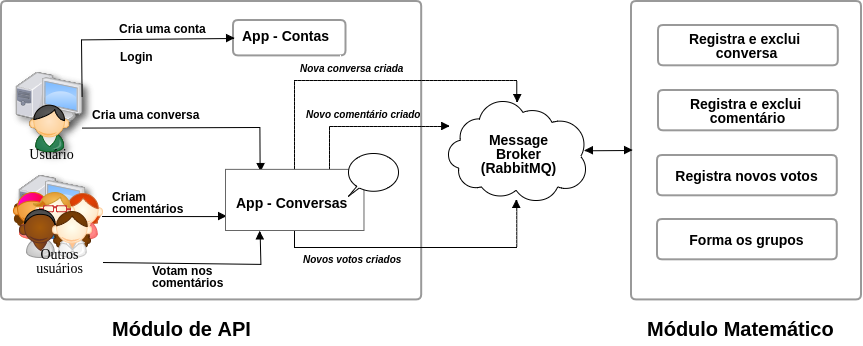
\includegraphics[scale=0.5]{figuras/resumo_ej_api.png}
	\caption{Funcionamento do Empurrando Juntos - Comunicação entre os módulos}
	\label{fig:resumo_ej_api}
	\end{figure}


	Na Figura \ref{fig:resumo_ej_api} é apresentado o fluxo de funcionamento do Empurrando Juntos de acordo com a arquitetura
	estabelecida e a API desenvolvida.
	
	Inicialmente, um usuário faz o cadastro e/ou autentica na aplicação,
	cuja requisição é tratada pelo \textit{app} de contas.
	Após a autenticação do usuário, ele pode criar conversas e comentários na aplicação.
	Outros usuários podem criar comentários e votar nos comentários.
	Todas essas operações relacionadas à conversas, comentários e votos
	são tratadas pelo \textit{app} de conversas.
	Quando uma nova conversa é criada, um novo comentário ou um novo voto é realizado
	em algum comentário de uma conversa, um sinal é disparado pelo \textit{app} de conversas
	para informar o ocorrido ao módulo matemático, enfileirando a tarefa correspondente
	no \textit{message broker}, via Celery.
	Essa chamada é recebida pelo \textit{message broker} que por sua vez delega
	a tarefa ao Celery do módulo matemático.
	Quando o número de votos configurado no sistema é atingido o \textit{app} de conversas
	faz uma chamada para a tarefa de clusterização que, ao ser recebida pelo módulo matemático,
	é a tarefa responsável por calcular os \textit{clusters} considerando o usuário do novo voto,
	gerando e retornando os novos grupos de usuários. Esse número de votos configurado é responsabilidade
	da implementação do módulo para poder gerenciar os momentos em que deve ser realizada clusterização visando 
	uma boa performance da aplicação.
	